\documentclass{standalone}

\usepackage{amsmath}
\usepackage{xparse}
\usepackage{my_commands}

\usepackage{tikz}
\usetikzlibrary{arrows}
\usetikzlibrary{positioning,decorations.pathreplacing,decorations.pathmorphing,arrows,fit}
\usetikzlibrary{calc}

\definecolor{darkgreen}{RGB}{0,128,80}


\begin{document}

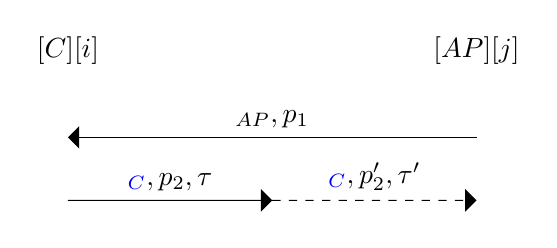
\begin{tikzpicture}
	\tikzset{
	    between/.style args={#1 and #2}{
	         at = ($(#1)!0.5!(#2)$)
	    }
	}
	
	\newcommand*{\CAspace}{4cm}
	\newcommand*{\MsgSpace}{0.8}

	\node[](C) {$\oracle[C][i]$};
	\node[right = \CAspace of C](A) {$\oracle[AP][j]$};
		

	\coordinate[below = \MsgSpace of C] (C1) {};
	\coordinate[below = \MsgSpace of A] (A1) {};
	\coordinate[between = C1 and A1] (M1) {};
	
	\coordinate[below = \MsgSpace of C1] (C2) {};
	\coordinate[below = \MsgSpace of A1] (A2) {};
	\coordinate[between = C2 and A2] (M2) {};

	\draw[triangle 90-] (C1) -- node[above] {$\nonce_{AP}, p_1$} (A1);
	\draw[-triangle 90] (C2) -- node[above] {$\textcolor{blue}{\nonce_C}, p_2, \tau$} (M2);
	\draw[-triangle 90,dashed] (M2) -- node[above] {$\textcolor{blue}{\nonce_C}, p_2', \tau'$} (A2);	
	
	
	\node[below=0pt of C2] {};
\end{tikzpicture}


\end{document}